\chapter{Impacts, risques et mesures}
\label{chapter:introduction}

\chapterabstract{Le changement climatique est à la fois extremement incertain, et nécessite des actions et des prises de décisions rapides et de grande envergure. Ce paradoxe a donné naissance à des institutions, comme le CCNUCC ou le GIEC, et à des outils, comme la modélisation intégrés. A chaque fois, l'objectif est de réduire l'incertitude et de favoriser le rapprochement entre l'action politique et la connaissance scientifique. Dans cette introduction, nous introduisons quelques uns des concepts cadres qui nous serons utiles tout au long du mémoire}

\newpage

%% Accroche
%Agir dans l'incertain : voici un des défis auquel nous soumet le changement climatique. L'action est nécessaire, tant l'ampleur de ces impacts est importante. Et l'incertitude est omniprésente : 

Les impacts du changement climatique sont de plus en plus présents dans le débat public : sécheresse, inondations, tempêtes font régulièrement les couvertures des journaux, et la plupart des partis politiques français ont pris position sur un programme climatique. C'est là une des spécificités du changement climatique : l'articulation très fine entre une réalité scientifique de plus en plus consensuelle d'une part, et de choix politiques incertains et normatifs d'autre part. 

%% Définition des termes

C'est justement la définition classique d'un risque : l'interaction entre un aléa et un enjeu. L'aléa, dans ce contexte, désigne un événement physique dont l'occurrence est possible : une canicule, un ouragan, la montée du niveau de la mer, etc. Un des effets du changement climatique est d'augmenter l'amplitude et la fréquence des aléas. L'enjeu est lié à ce que l'on a à perdre, c'est-à-dire ce qui a de la valeur et qui peut être affecté par la réalisation de l'aléa. 

%% Rappel du sujet
Nous nous intéressons au rôle des fonctions de dommage dans la formation de ces décisions politiques. 



%% Problématique
Nous tenterons ici de donner des éléments de contexte à la question suivante : 
Comment les fonctions de dommage des modèles intégrés permettent-elles de prendre en compte les risques climatiques ? Celle-ci s'accompagne d'autres questions : Quels sont les risques climatiques ? Comment sont pris en compte ces risques dans la gouvernance mondiale et nationale ? Et quels outils permettent d'éclairer ces prises de décision ? 



%% Annonce du plan 
Ce chapitre est construit en trois parties. Dans une première partie, nous nous intéresserons aux impacts du changement climatique, en les classant en trois types : les effets de tendance, qui sont linéaires ; les effets ponctuels et catastrophiques ; et les effets de seuil, ou tipping points. Nous aborderons dans une deuxième partie la manière dont les institutions internationales se sont organisées pour faire face à ces risques, et comment ces questions articulent des composantes scientifiques et politiques. Enfin, dans une troisième partie, nous détaillerons certains des outils qui ont été développés pour répondre à ces enjeux : les modèles intégrés, leurs fonctions de dommage et le coût social du carbone. 




\section{Le changement climatique : tendances et impacts}
\label{sect/1/1}

Cette section décrit les impacts du changement climatique et la manière de les prendre en compte

\subsection{Les effets moyens}
\label{sect/1/1/1}

% Presenter les rapports du GIEC

Présenter ici les rapports du Giec. a la différence des tipping points

\subsection{Les catastrophes}
\label{sect/1/1/2}

\subsection{Les tipping points}
\label{sect/1/1/3}

\begin{figure}
    \centering
    %\includegraphics{}
    \caption{Après un point de bascule, la dynamique du système change radicalement. \textit{Les tipping points, comme les événements catastrophiques, sont plus difficiles à modéliser que la tendance moyenne des dommages. }}
    \label{fig:tipping-point}
\end{figure}

Les points de bascule, ou tipping points, sont des évolutions d'un système sous lequel celui-ci se comporte différemment. 

\paragraph{Les risk tipping points}

Au-delà de la définition classique du tipping point, l'Université des Nations Unies propose, dans son rapport sur les risques interconnectés, une nouvelle définition des risques interconnectés. Un \textit{risk tipping point}, ou point de bascule des risques, désigne \textit{l'instant où un système socioécologique ne peut plus absorber le risque et réaliser ses fonctions}. Après le passage de ce point de bascule, la possibilité d'un impact catastrophique augmente substantiellement. Six risques sont identifiés comme particulièrement représentatif des effets systémiques d'un driver sur tous les autres : l'accélération de l'extinction de la biodiversité, la réduction de l'eau de surface disponible, la fonte des glaciers, les débris spatiaux, la chaleur trop importante, et un futur qui n'est plus assurable. Parmi ces points de bascule, quatre sont  reliés à l'augmentation de la température atmosphérique ou océanique, et quatre à l'augmentation de la concentration en gaz à effet de serre dans l'atmosphère. \cite{united_nations_university_-_institute_for_environment_and_human_security_unu-ehs_interconnected_2023}

Ce concept est intéressant pour deux raisons : d'abord, il illustre la complexité des systèmes physiques et sociaux, et la complexité de leur interaction. Ensuite, il montre que la prise en compte d'un impact par le moyen d'un seul mécanisme risque de sous-estimer cet impact, car cela ne permet pas de prendre en compte les réactions en chaines et les interactions entre les différents impacts. 

\section{Prendre des décisions dans l'incertain : le rapprochement de la science et du pouvoir}
\label{sect/1/2}


Ressource : gouverner le climat

\subsection{Historique des négociations climatiques}
\label{sect:1.2.1}

\subsection{Le cadre général : CCNUCC et COP}
\label{sect:1.2.2}
Faire un retour de l'histoire des COP, de la CCNUCC 

\subsection{La synthèse des connaissances actuelles : le GIEC}
\label{sect:1.2.3}

\subsection{Loss and damages : dommages, responsabilité et évaluation}
\label{sect:1.2.4}

\section{Les outils : de la modélisation intégrée}
\label{sect:1.3}

Un des outils phare développé pour comprendre le changement climatique sont les \gls{iam}.

\subsection{Les modèles intégrés, ou comment cartographier les dynamiques du monde}
\label{sect:1.3.1}

Se baser beaucoup sur l'article de Cointe 2024 + Gouverner le climat \\

La modélisation intégrée a pris beaucoup de place au fur et à mesure que le giec a pris de l'importance

\subsection{Le coût social du carbone}
\label{sect:1.3.2}

\begin{figure}
    \centering
    %\includegraphics{}
    \caption{Estimations des coûts sociaux du carbone. \textit{Depuis 30 ans, les agences fédérales des États-Unis doivent inclure le coût social du carbone dans leurs études d'impact. Celui-ci est estimé à partir de trois modèles intégrés : RICE, FUND et PAGE. Sa valeur est très sensible du taux d'actualisation.}}
    \label{fig:scc}
\end{figure}

\subsection{Les fonctions de dommage}
\label{sect:1.3.3}

\begin{figure}
    \centering
    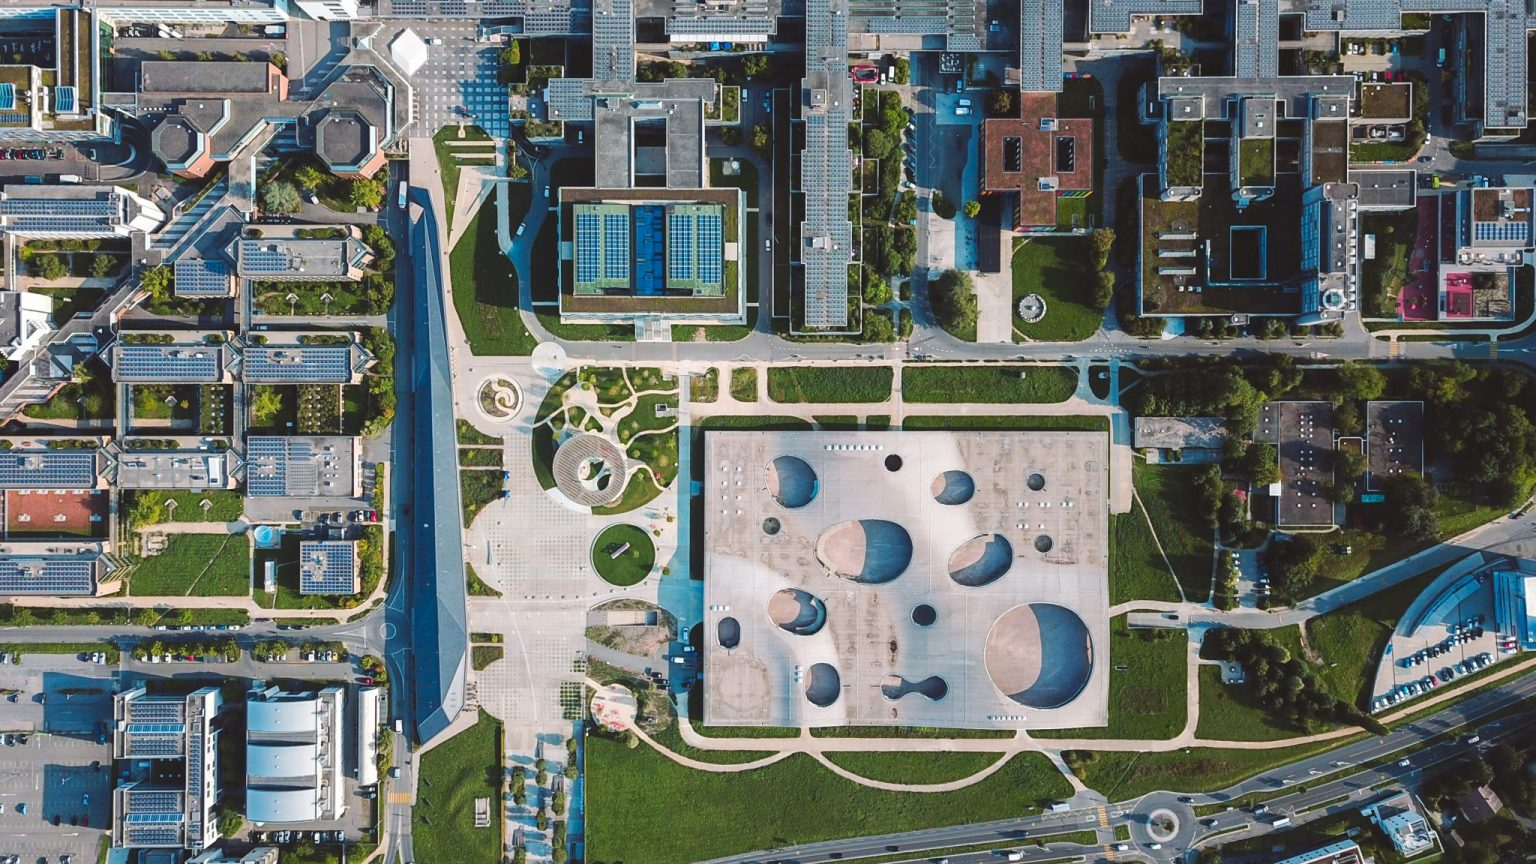
\includegraphics[width=4cm]{figures/campus.jpg}
    %\begin{tikzpicture}[scale=1]

\def\figureheight{20} % Choisis la hauteur désirée
\def\nodedistance{\textwidth*1/3}
\def\verticaldistance{2cm}
\def\nodewidth{3cm}

% Trajectory
\draw[line width = 2pt, rounded corners=8pt] (0,0) -- node[midway, below]{Les premières intuitions} (\textwidth,0) -- (\textwidth,-\figureheight*1/3) -- node[midway, below]{L'essor de la climatologie}(0,-\figureheight*1/3) -- (0,-\figureheight*2/3) -- node[midway, below]{Naissance du \textit{régime climatique}}(\textwidth,-\figureheight*2/3);


% Phase 1 : les premières intuitions


\node (1822) at (0,0.5) {1822};
\node (fourrier) [rectangle, draw, above of = 1822, text width=\nodewidth, text centered, yshift=2cm]{
Fourrier théorise l'effet de serre \\
\includegraphics[width=\linewidth]{images/Fourier2.jpg}
};

\node (1859) [right of = 1822, node distance = \nodedistance] {1859};
\node (tyndall) [rectangle, draw, above of=1859, text width=\nodewidth, text centered]{John Tyndall};

\node (1896) [right of = 1859, node distance = \nodedistance] {1896};
\node (farrhenius) [rectangle, draw, above of=1896, text width=\nodewidth, text centered]{Svante Arrhenius};

\node (1938) [right of = 1896, node distance = \nodedistance] {1938};
\node (callendar) [rectangle, draw, above of=1938, text width=\nodewidth, text centered]{Guy Callendar};

% 1822 : Joseph Fourrier
% 1859 : John Tyndall
% 1896 : Svante Arrhenius
% 1938 : Guy Callendar


% Phase 2 : l'essor de la climatologie

% Phase 3 : l'essor du régime climatique


% Information boxes
\draw[fill=blue!20] (0.5,-1) rectangle (2.5,-2);
\node at (1.5,-1.5) {Création du GIEC};
\draw[fill=green!20] (7.5,-1) rectangle (9.5,-2);
\node at (8.5,-1.5) {Première COP};
% Add more information boxes as needed
\end{tikzpicture}
    \caption{Évolution jointe de la modélisation et des négociations climatiques. \textit{Les modèles climatiques ont permis en premier de concevoir et de détecter le changement climatique (A). Leur essor a accompagné le cadrage de la question climatique (B), et ils sont désormais un outil de prise de décision (C).}}
    \label{fig:frise}
\end{figure}

\ref{sect/1/1}


